\documentclass[]{article}

\usepackage[a4paper, top=2in, bottom=1.5in, left=1in, right=1in]{geometry}
\usepackage{amsmath}
\usepackage{amssymb}
\usepackage{graphicx}
\usepackage{float}

\setlength{\parindent}{0cm}

\begin{document}

\title{\textbf{Complexiteitstheorie} \\ Bullet points en dat soort dingen \\ ~ \\ \texttt{``sharing is caring''} \\ ~}
\author{Hylke Visser \\ \textit{hylkev@ch.tudelft.nl}}
\date{}
\maketitle

\renewcommand{\abstractname}{}

\begin{abstract}
De volgorde van de onderwerpen in dit document komt overeen met de volgorde waarin deze onderwerpen tijdens de colleges in 2014 zijn behandeld. Aanpassingen of toevoegingen aan dit document: \texttt{https://github.com/hylkev/complexiteitstheorie-bullet-points} \\ $~$ \hfill \textit{Laatste update: \today}
\end{abstract}

\section*{Basiskennis}

\begin{description}
\item[Tijdcomplexiteit:] $f : N \rightarrow N$ waarbij $f(n)$ het grootste aantal stappen is dat M nodig heeft voor een input van grootte $n$.
\item[Complexiteit van een probleem:] de \textit{worst-case complexiteit} van het beste algoritme, uitgevoerd op het gekozen machinemodel.
\item[Relaties tussen Tm's:] Voor elke \textit{k-tape} ($k \geq 2$) DTm die een probleem oplost in $t(n)$-tijd, bestaat er een \textit{single-tape} DTm die hetzelfde probleem oplost in O($t^2(n)$)
\item[Sterke Church-Turing these:] Elk fysisch realiseerbaar algoritmisch proces kan worden gesimuleerd op een 1-tape DTm met \textit{polynomiale overhead} (met mogelijke uitzondering de quantum computer).
\item[Complexiteitsklasse (N)TIME(t(n)):] Verzameling van alle talen beslist door O($t(n)$)-(N)DTm's.
\end{description}

\section*{Tijd-hierarchie}

\textbf{TIME($f(n)$) $\subseteq$ NTIME($f(n)$)}

\bigskip

\begin{description}
\item[TIME($\mathbf{1}$)]
\item[TIME(log(n))]
\item[TIME($\mathbf{\sqrt n}$)]
\item[TIME($\mathbf{n}$)] Lineair
\item[TIME(n $\cdot$ log(n))]
\item[TIME($\mathbf{n^c}$)] Polynomiaal
\item[TIME($\mathbf{n^{log(n)}}$)] Quasi-polynomiaal
\item[TIME($\mathbf{2^{\sqrt n}}$)] Subexponentieel
\item[TIME($\mathbf{2^{O(n)}}$)] Exponentieel
\end{description}

\section*{Doenlijk vs Ondoenlijk}
Een probleem is doenlijk als het in polynomiale tijd op te lossen is. Een probleem is ondoenlijk als er geen polynomiaal algoritme voor het probleem bestaat. Technologische vooruitgang heeft een positieve invloed op de snelheid waarmee doenlijke problemen kunnen worden opgelost. Bij ondoenlijke problemen is technologische vooruitgang niet van belang.

\section*{Complexiteitsklassen}

Hi\"erarchie: P $\subseteq$ NP $\subseteq$ EXP.

\section*{P}

\begin{itemize}
\item Talen die door een DTm in polynomiale tijd beslist worden.
\item $\bigcup_{k\geq 0} \text{TIME}(n^k)$
\end{itemize}

\section*{NP}

\begin{itemize}
\item Talen die door een NDTm in polynomiale tijd beslist worden.
\item $\bigcup_{k\geq 0} \text{NTIME}(n^k)$
\item Talen die door een DTm in polynomiale tijd geverifieerd worden.
\begin{itemize}
\item Met behulp van een certificaat $c$
\end{itemize}
\item Het is onbekend of P = NP of P $\not=$ NP
\end{itemize}

\section*{Polynomiale Reducties}

\begin{itemize}
\item Als een probleem A reduceerbaar is tot een probleem B (A $\leq$ B), kan een effici\"ente oplossing voor B gebruikt worden voor het efficient oplossen van A.
\item Een reductiefunctie $f : \Sigma^* \rightarrow \Sigma^{'*}$ transformeert een probleem A naar probleem B.
\item $w \in$ A $\Leftrightarrow f(w) \in$ B
\begin{itemize}
\item yes-instanties van A worden afgebeeld op yes-instanties van B
\begin{itemize}
\item $\forall x \in \Sigma^* : x \in A \rightarrow f(x) \in B$
\end{itemize}
\item no-instanties van A worden afgebeeld op no-instanties van B
\begin{itemize}
\item $\forall x \in \Sigma^* : x \not\in A \rightarrow f(x) \not\in B$
\item $\forall x \in \Sigma^* : f(x) \in B \rightarrow x \in A$
\end{itemize}
\end{itemize}
\item $f$ is polynomiaal berekenbaar.
\item Als A$_\text{B}$ een polynomiaal algoritme is voor $B$, dan is A$_\text{B}$ $\circ$ $f$ een polynomiaal algoritme voor A.
\item Dan geldt dat A \textit{niet essentieel moeilijker is dan B}.
\end{itemize}

\begin{description}
\item[P is naar beneden gesloten onder $\leq$] ~ \\
Als $f$ een polynomiale-tijd reductie is van A naar B (A $\leq$ B), dan geldt: als B $\in$ P dan A $\in$ P
\item[Eigenschappen van polynomiale reducties] ~ \\
Reflexiviteit, Transitiviteit
\end{description}

\section*{Correctheid van Reducties bewijzen}

\begin{itemize}
\item Bewijs de betrouwbaarheid van $f$
\begin{itemize}
\item yes-instanties van A $\rightarrow$ yes-instanties van B
\item no-instanties van A $\rightarrow$ no-instanties van B
\end{itemize}
\item Bewijs de polynomialiteit van $f$
\end{itemize}

\section*{NP-hard en NP-compleet (NPC)}

Een probleem B is NP-hard (onder $\leq$) als voor iedere X in NP geldt dat X $\leq$ B.

Een probleem A is NP-compleet (onder $\leq$) als geldt dat:

\begin{itemize}
\item A $\in$ NP
\item A is NP-hard (onder $\leq$)
\end{itemize}

\begin{description}
\item[P] bevat de eenvoudigste problemen in NP
\item[NPC] bevat de moeilijkste problemen in NP
\item[Als P $\not=$ NP] bevat NP oneindig veel verschillende moeilijkheidsniveaus
\item[Als A $\in$ NPC, B $\in$ NP en A $\leq$ B] dan B $\in$ NPC.
\item[Als A $\in$ NPC $\cap$ P] dan P = NP
\item[Als A $\in$ NPC en A $\not\in$ P] dan P $\not=$ NP
\end{description}

\section*{A $\in$ NPC bewijzen}

\begin{itemize}
\item Bewijs dat A $\in$ NP
\begin{itemize}
\item Toon aan dat het probleem polynomiaal verifieerbaar is
\end{itemize}
\item Bewijs dat B $\leq$ A voor een bekend NPC probleem B
\begin{itemize}
\item Kies een geschikt bekend NPC probleem B
\item Construeer een polynomiale reductie B $\leq$ A
\item Bewijs de correctheid van deze reductie
\end{itemize}
\end{itemize}

\section*{co-NP}

\begin{itemize}
\item Het complement van een probleem A is het probleem A$^\text{c} = \Sigma^* - $ A
\item co-NP bestaat uit alle problemen B die het complement zijn van een probleem A in NP
\item co-NP = \{ B : $\exists$ A $\in$ NP [ B = A$^\text{c}$ ] \}
\item A in co-NP als een NDTm no-instanties in polynomiale tijd oplost
\item A in co-NP als no-instanties polynomiaal verifieerbaar zijn
\end{itemize}

\begin{description}
\item[Als A $\leq$ B] dan A$^\text{c}$ $\leq$ B$^\text{c}$
\item[Als A $\in$ NPC] dan A$^\text{c}$ $\in$ co-NPC
\end{description}

\begin{figure}[H]
\centering
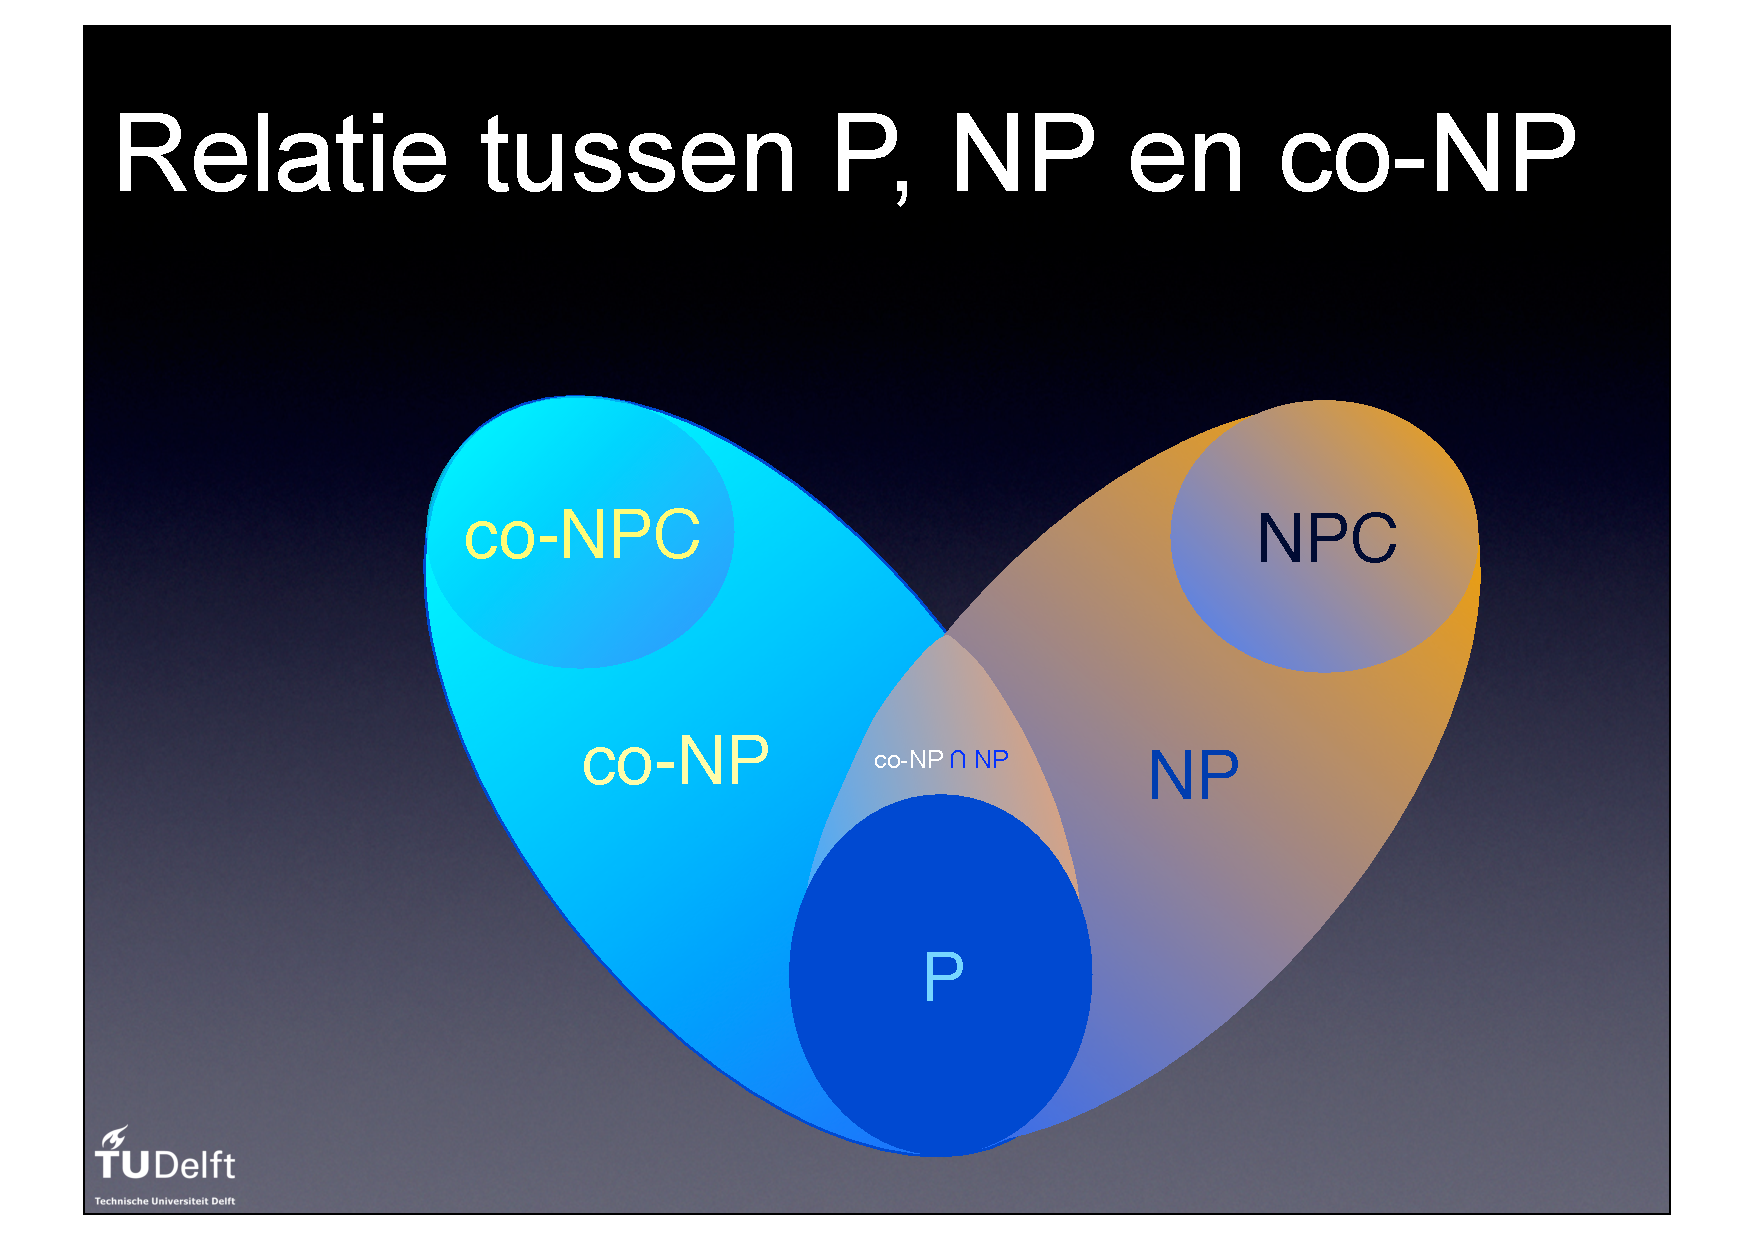
\includegraphics[width=0.6\columnwidth]{slides/p-np-co-np}
\end{figure}

\section*{Bewijs met restrictie}
Een beslissingsprobleem A is een restrictie van een probleem B als:

\begin{itemize}
\item Yes$_\text{A}$ $\subseteq$ Yes$_\text{B}$
\item No$_\text{A}$ $\subseteq$ No$_\text{B}$
\end{itemize}
NB: het omgekeerde geldt niet, dit is een verschil met reductie.

\begin{description}
\item[Als probleem A een restrictie is van B] dan kan ieder algoritme voor probleem B gebruikt worden om probleem A op te lossen, er geldt A $\leq$ B.
\end{description}

Om aan te tonen dat B een NP-compleet probleem is:

\begin{itemize}
\item Bewijs dat B $\in$ NP
\item Bewijs dat een bekend NP-hard probleem A een restrictie is van B
\end{itemize}

Een voorbeeld van restrictie is PARTITION, wat een restrictie van SUBSUM is met $t = \lfloor (\sum_{s \in S} s) / 2 \rfloor$.

\section*{Ruimtecomplexiteit}

\begin{description}
\item[SPACE($f(n)$)] \{ L : L wordt geaccepteerd door een DTm die O($f(n)$) ruimte gebruikt \}
\item[NSPACE($f(n)$)] \{ L : L wordt geaccepteerd door een NDTm die O($f(n)$) ruimte gebruikt \}
\end{description}

\medskip

\textbf{SPACE($f(n)$) $\subseteq$ NSPACE($f(n)$)}

\medskip

\begin{description}
\item[PSPACE] = $\bigcup_{k \geq 0}$ SPACE($n^k$)
\begin{description}
\item[L] = SPACE(log n)
\item[PolyL] = $\bigcup_{k \geq 0}$ SPACE(log$^\text{k}$ n)
\end{description}

\medskip

\item[NPSPACE] = $\bigcup_{k \geq 0}$ NSPACE($n^k$)
\begin{description}
\item[NL] = NSPACE(log n)
\item[PolyNL] = $\bigcup_{k \geq 0}$ NSPACE(log$^\text{k}$ n)
\end{description}
\end{description}

\medskip

\textbf{P $\subseteq$ NP $\subseteq$ PSPACE}

\textbf{PSPACE = NPSPACE}

\section*{PSPACE-hard en PSPACE-compleet}

Een probleem is PSPACE-compleet als:

\begin{itemize}
\item A $\in$ PSPACE
\item X $\leq$ A voor elk PSPACE probleem X
\end{itemize}

\section*{Getalproblemen en Pseudo-polynomiale algoritmen}

\begin{description}
\item[$I_A$:] instantie van probleem $A$
\item[$|I_A|$:] grootte van $I_A$
\item[max($I_A$):] grootte van het grootste getal in $I_A$ (unaire codering)
\end{description}

$A$ is een getalprobleem als er geen enkele polynoom $p(~)$ bestaat zodat voor alle instanties $I_A$ geldt dat max($I_A$) $\leq$ $p(|I_A|)$

\medskip

Een algoritme X$_\text{A}$ voor een getalprobleem $A$ is een pseudo-polynomiaal algoritme als de tijdcomplexiteit van X$_\text{A}$ gelijk is aan $O(q(|I_A|, \text{max}(I_A)))$ voor een polynoom q(~,~) en voor alle instanties $I_A$ van A.

\section*{Sterk NP-complete problemen}

$A_p$: het subprobleem van A bestaande uit instanties $I_A$ met kleine getallen: \\
max($I_A$) $\leq$ p($|I_A|$)

A is sterk NP-compleet (SNPC) als:

\begin{itemize}
\item A $\in$ NP
\item er bestaat een polynoom p met $A_p \in$ NPC
\end{itemize}

\textbf{Oftewel,} de grootte van de getallen is niet van invloed op de moeilijkheid van het probleem

\section*{Tijd en ruimte construeerbaar / separatie}

\begin{itemize}
\item Hoveel moet de hoeveelheid tijd of geheugen toenemen om een verschil te maken?

\item Een functie $f:N \rightarrow N$ is ruimte-construeerbaar als er een DTM bestaat die voor input $1^n$ als output $[f(n)]_2$ berekent in O(f(n))-ruimte.

\item Een functie $f:N \rightarrow N$ is tijd-construeerbaar als er een DTM bestaat die voor input $1^n$ als output $[f(n)]_2$ berekent in O(f(n))-tijd.

\end{itemize}

\textbf{Gevolg:}

\begin{figure}[H]
\centering
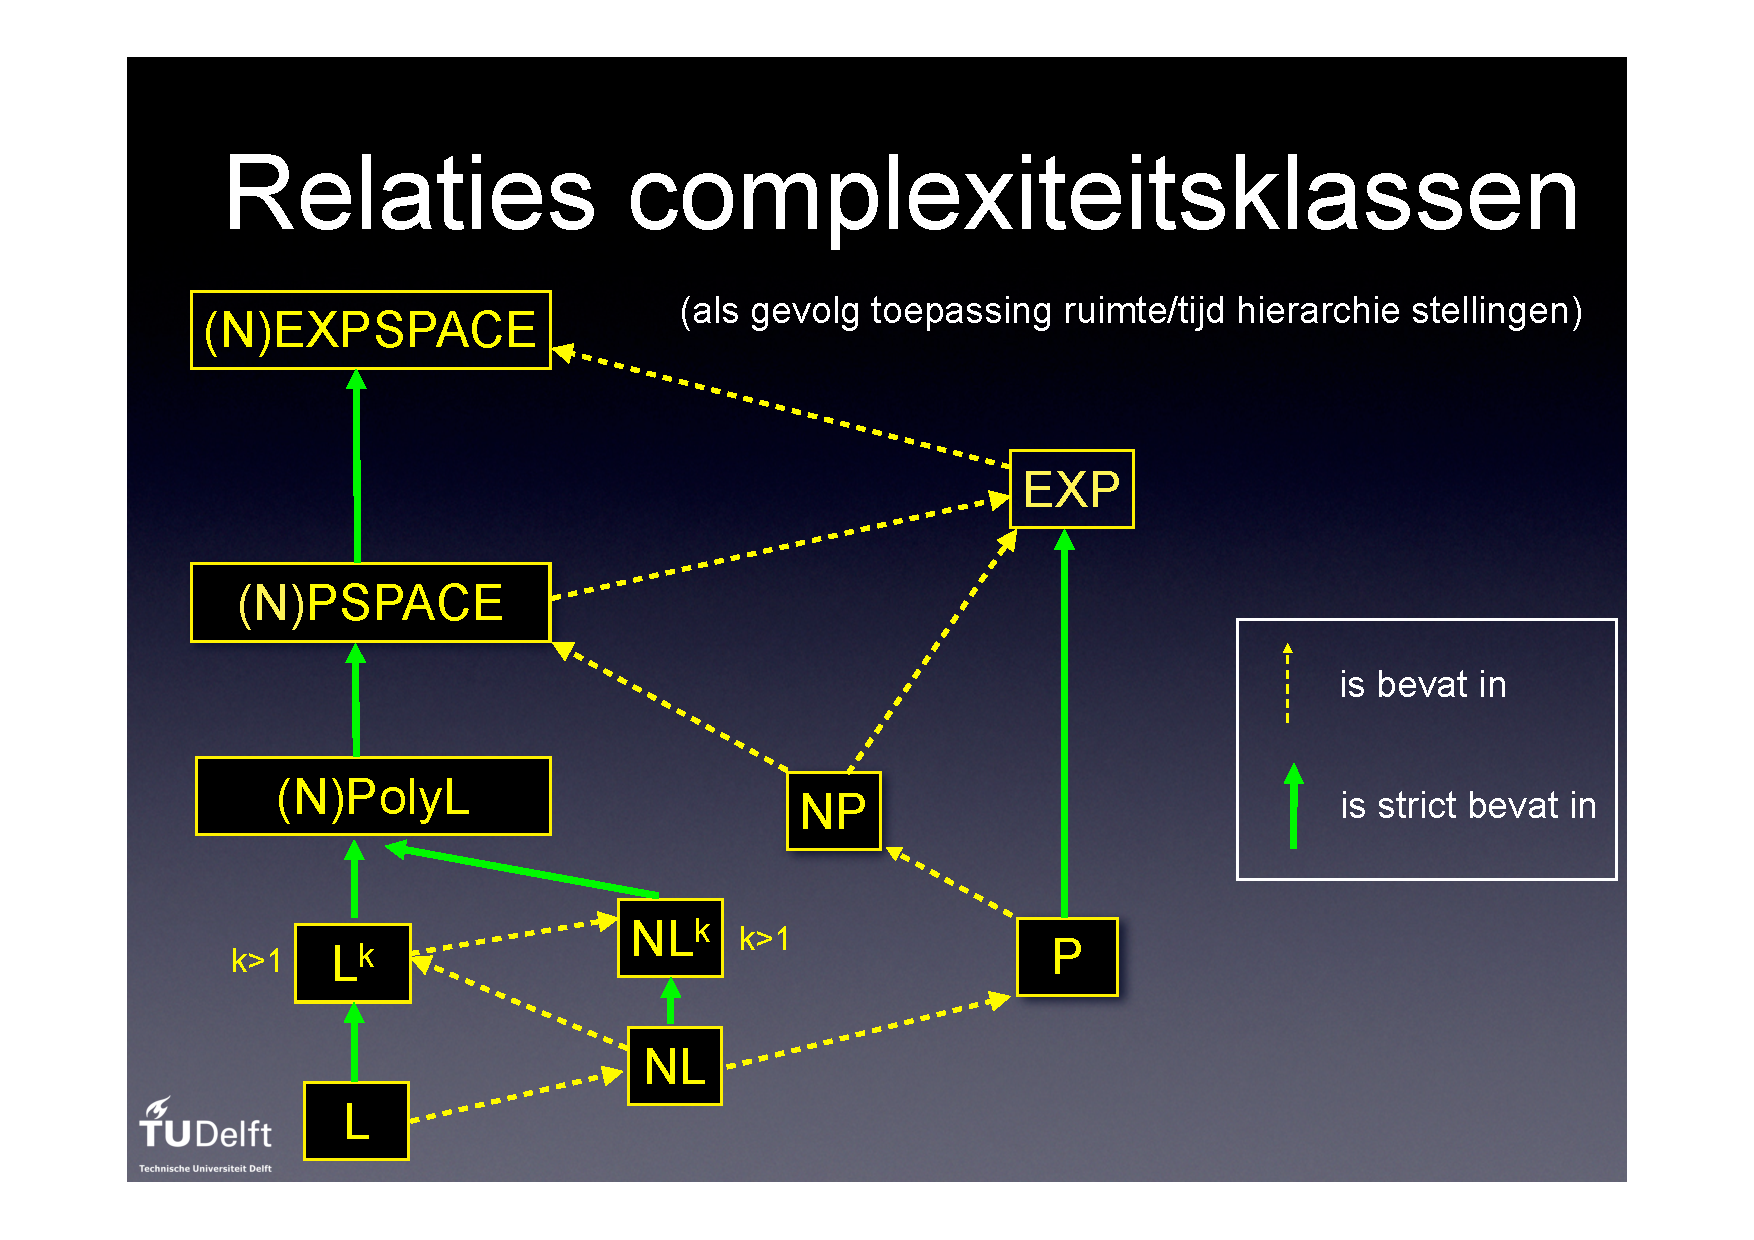
\includegraphics[width=0.6\columnwidth]{slides/relaties}
\end{figure}

\section*{Orakels / Relativized Complexity Classes}

\begin{description}
\item[$\mathbf{C^Y}$] bevat talen die een C algoritme hebben als een Y orakel wordt gebruikt
\item[$\mathbf{P^{NP}}$] bevat talen die polynomiaal beslisbaar zijn door gebruik van een NP orakel 
\item[$\mathbf{NP^{NP}}$] bevat talen die polynomiaal verifieerbaar zijn door gebruik van een NP orakel 
\item[$\mathbf{co-NP^{NP}}$] bevat talen waarvan het complement verifieerbaar is in polynomiale tijd door gebruik van een NP-orakel
\end{description}

\begin{figure}[H]
\centering
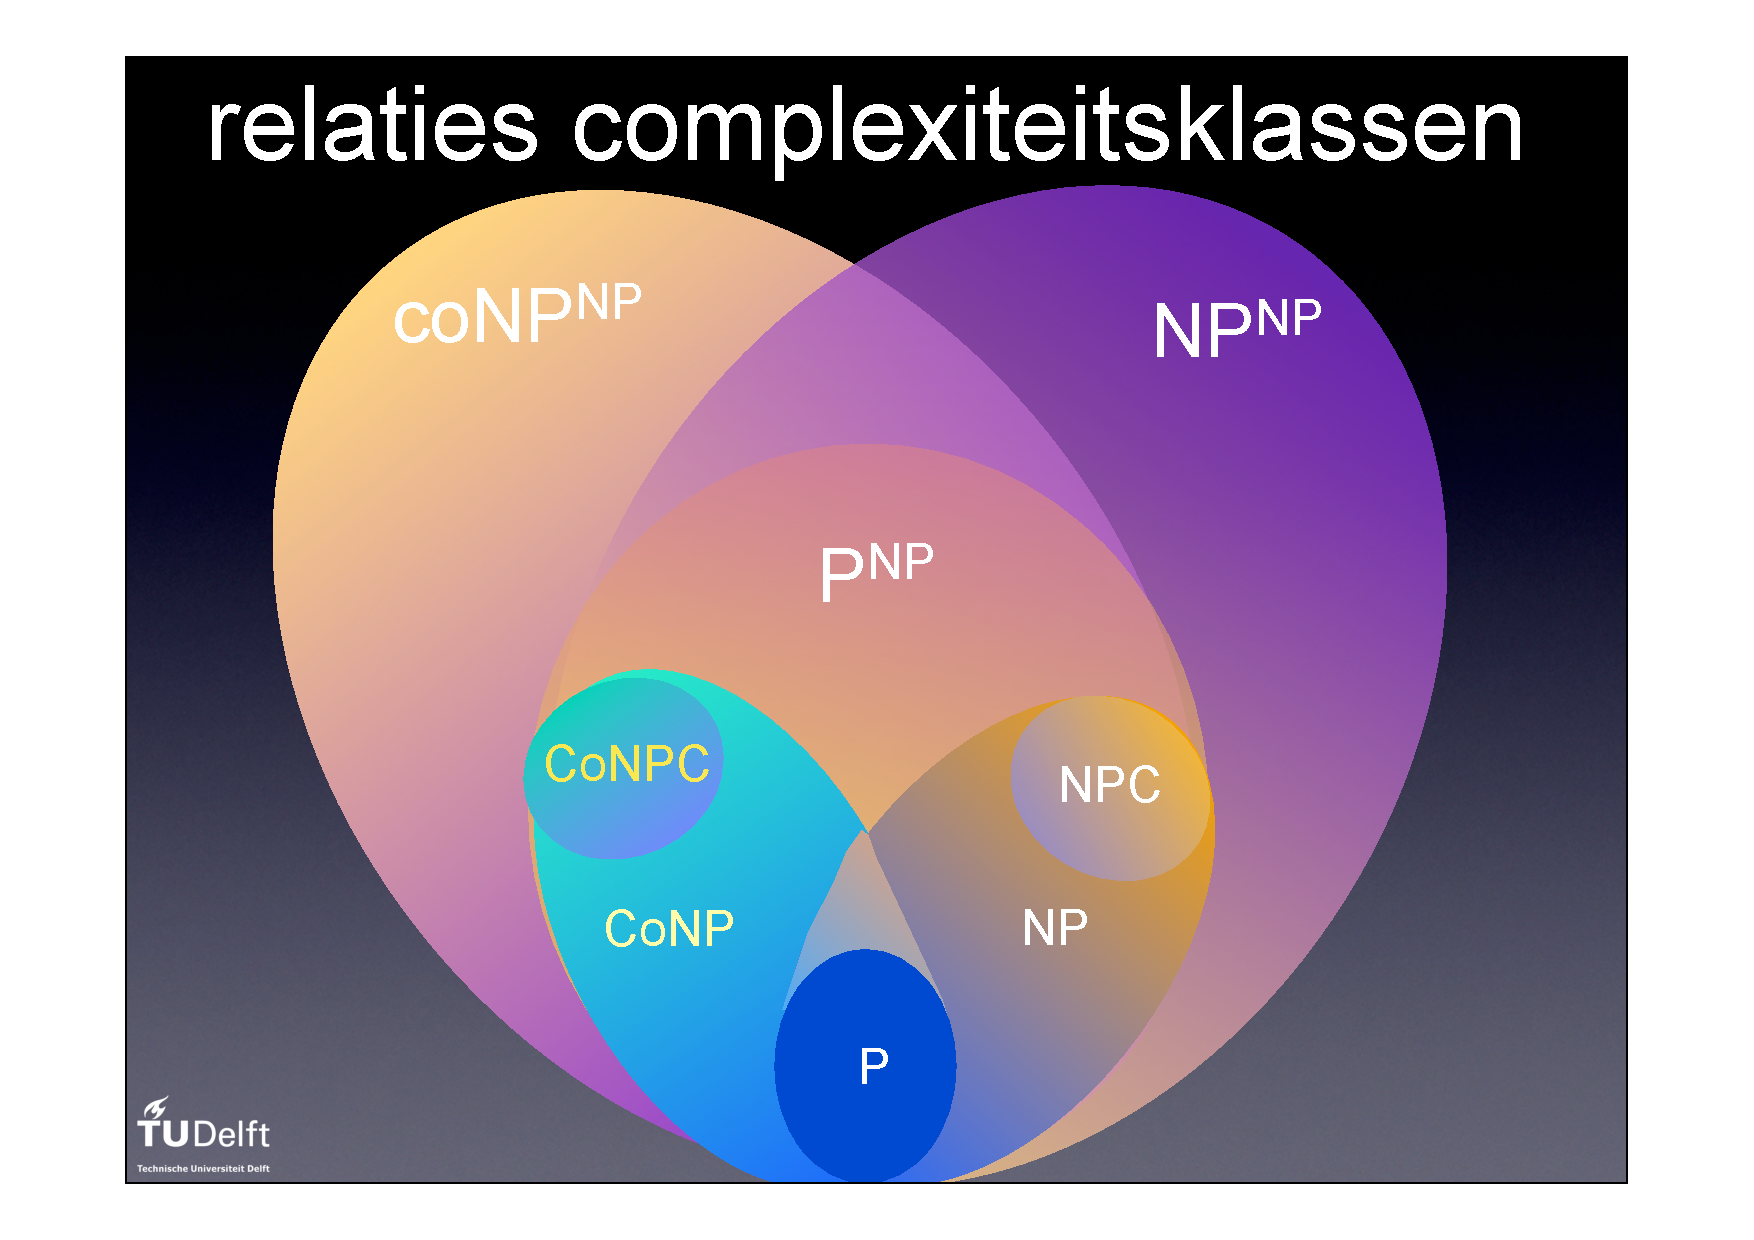
\includegraphics[width=0.6\columnwidth]{slides/orakel-klassen}
\end{figure}

\section*{Zero Knowledge Proof Systems}

\textbf{P}\textit{rover} wil \textbf{V}\textit{erfifier} ervan overtuigen dat \textbf{P} in het bezit is van informatie X, zonder de inhoud van X aan \textbf{V} prijs te geven.

\begin{description}
\item[Completeness:] if the statement is true, the honest verifier (that is, one following the protocol properly) will be convinced of this fact by an honest prover.
\item[Soundness:] if the statement is false, no cheating prover can convince the honest verifier that it is true, except with some small probability.
\item[Zero-knowledge:] if the statement is true, no cheating verifier learns anything other than this fact. This is formalized by showing that every cheating verifier has some simulator that, given only the statement to be proven (and no access to the prover), can produce a transcript that ``looks like'' an interaction between the honest prover and the cheating verifier.
\end{description}

\section*{Optimaliseringsproblemen}

\begin{description}
\item[Decisie (dec):] Gegeven een instantie x, een integer $d$ en een kostenfunctie $c(~)$, is er een oplossing $y$ van x met kosten $c(y) > d$ (of $c(y) < d$)?
\item[Optimalisatie (opt):] Gegeven een instantie x en een kostenfunctie $c(~)$, bepaal een oplossing $y$ van $x$ met minimale/maximale kosten $c(y)$.
\item[Optimal value (val):] Gegeven een instantie x en een kostenfunctie $c(~)$, bepaal de minimale/maximale kosten $c(y)$ haalbaar voor een oplossing $y$ van $x$.
\end{description}

\textbf{Kenmerken:}

\begin{itemize}
\item Voor elke instantie $x \in A$ is er een verzameling $F(x)$ van mogelijke oplossingen (feasible solutions).
\item De kostenfunctie $c(~)$ bepaalt voor iedere $y \in F(x)$ de kosten $c(y)$ van $y$.
\item Er is een optimale oplossing opt$(x) \in F(x)$ met minimale (of maximale) kosten.
\begin{itemize}
\item Vaak wordt opt$(x)$ ook gebruikt om de kosten van de optimale oplossing aan te geven
\end{itemize}
\end{itemize}

Een optimaliseringsprobleem $A$ is een \textbf{NPO-probleem} (Niet-Deterministisch Polynomiaal Optimaliseringsprobleem) als:

\begin{enumerate}
\item voor elke $y \in F(x)$ geldt dat $|y|$ polynomiaal begrensd is in $|x|$
\item voor elke $x \in A$ is het probleem $y \in F(x)$? een P-probleem (als 1.)
\item voor elke $y \in F(x)$ is $c(y)$ polynomiaal berekenbaar
\end{enumerate}

\section*{Turing Reducties}

$A \leq_\text{T} B$: Er is een algoritme voor A dat orakelaanroepen voor B gebruikt en polynomiaal zou zijn als orakelaanroepen O(1)-tijd kosten.

\begin{itemize}
\item $A \leq_\text{T} A$
\item Als $A \leq_\text{T} B$ en $B \leq_\text{T} C$, dan $A \leq_\text{T} C$
\end{itemize}

en

\begin{itemize}
\item A-dec $\leq_\text{T}$ A-opt
\item A-val $\leq_\text{T}$ A-dec
\item A-opt $\leq_\text{T}$ A-val als A zelf-reduceerbaar is (A-dec $\in$ NPC)
\end{itemize}

\bigskip

Een (optimaliserings, value, decisie) probleem A-opt is

\begin{itemize}
\item \textbf{NP-hard} als $\forall B \in \text{NP}, B \leq_\text{T} A$
\item \textbf{NP-easy} als $\exists B \in \text{NP}, A \leq_\text{T} B$
\item \textbf{NP-equivalent} als $A \in$ NP-hard $\cap$ NP-easy
\end{itemize}

\bigskip

Als A-dec $\in$ (co)NPC, dan:
\begin{itemize}
\item A-opt $\in$ NP-equivalent
\item A-val $\in$ NP-equivalent
\end{itemize}

\section*{Approximatie algoritmen}

\textbf{Een approximatie algoritme geeft altijd een feasible oplossing, maar niet noodzakelijk een optimale.}

\medskip

Performance ratio van M voor een instantie $x \in A$:
\[
R_\text{M}(x) = {{ \text{max} \{ \text{opt}(x), c(M(x)) \} } \over { \text{min} \{ \text{opt}(x), c(M(x)) \} }}
\]
Dit is altijd een getal $\geq$ 1; hoe dichter bij 1 hoe beter.

\medskip

M wordt een $r$-approximatie algoritme voor A genoemd als de performance ratio $R_\text{M}(x)$ voor iedere instantie $x$ kleiner of gelijk is aan $r$

\[
\forall x ~ R_\text{M}(x) \leq r
\]

\medskip

\textbf{$\mathbf{A} \in$ APX:} Een NPO-probleem A is goed-benaderbaar als er een polynomiaal c-approximatie algoritme voor A bestaat met $c < \infty$.

\section*{Boolese Circuits}

Een boolese circuit $C_m$ bestaat uit $m+n$ knopen (poorten/gates) verbonden door lijnen (wires). De eerste $m$ poorten zijn input poorten, de overige $n$ poorten zijn circuit poorten. Iedere poort is een boolese functie $\wedge, \vee, \neg$.

\begin{description}
\item[size(C):] aantal poorten van C
\begin{itemize}
\item bepaalt de sequentiele tijd van berekeningen
\end{itemize}
\item[depth(C):] langste pad van input naar output
\begin{itemize}
\item bepaalt de parallelle tijd van berekeningen
\end{itemize}
\end{description}

Een \textbf{circuit familie} $C$ is een oneindige lijst ($C_1, ..., C_m, ...$) van circuits $C_m$; iedere $C_m$ heeft $m$ input variabelen.

\medskip

Als $t$ een superlineaire functie is ($t(n) \geq n$), dan geldt: \\
\hspace*{1cm} als $A \in TIME(t(n))$ dan heeft A een circuit size complexiteit $O(t^2(n))$

\medskip

Een probleem is efficient parallelliseerbaar als het kan worden opgelost (\textbf{NC} / Nick's Classes):

\begin{itemize}
\item in extreem korte berekeningstijd
\begin{itemize}
\item poly-logaritmische tijd
\item depth = $O(\log^{O(1)}n)$
\end{itemize}
\item met een redelijk aantal processoren
\begin{itemize}
\item polynomiaal begrensd aantal processoren
\item size = $O(n^{O(1)})$
\end{itemize}
\end{itemize}

\textbf{NC$^i$} is de klasse van problemen die kunnen worden opgelost met een familie van circuits waarvoor geldt dat:

\begin{itemize}
\item size(C) = $n^{O(1)}$
\item depth(C) = O($\log^i n$)
\end{itemize}

\textbf{NC} is de klasse \{ A $ | ~ \exists i$. A $\in$ NC$^i$ \}

\medskip

Een NC-algoritme is een algoritme dat in O($\log^O(1)$)-tijd en met O($\log^O(1)$)-processoren kan worden uitgevoerd.

\medskip

NC $\subseteq$ P

\medskip

Een probleem A is P-compleet als
\begin{itemize}
\item $A \in P$
\item voor iedere $B \in P$ geldt $B \leq_\text{NC} A$
\end{itemize}

\medskip 

Problemen in P - NC worden inherent sequentieel genoemd.

Voor deze problemen zijn geen effici\"ente parallelle algoritmen gevonden.

\section*{Probablistische Algoritmen}

Een probabilistisch algoritme is een algoritme dat naast de input x een random source gebruikt om tijdens de executie random keuzes te maken.

\medskip

Voordelen:
\begin{itemize}
\item Efficientie
\item Eenvoudig ontwerp
\item Inspiratiebron voor deterministisch algoritme
\end{itemize}

\medskip

Een Probablistische Turing Machine (PTm) is een speciale NDTm waarbij in iedere configuratie een probablistische keuze gemaakt wordt uit de twee mogelijk toepasbare instructies.

\medskip

Een taal L wordt geaccepteerd door een PTm M met foutmarge $\varepsilon$ als
\begin{itemize}
\item $x \in L$ impliceert Pr[M accepteert x] $\geq 1 - \varepsilon$
\item $x \not\in L$ impliceert Pr[M verwerpt x] $\geq 1 - \varepsilon$
\end{itemize}

\medskip

\textbf{Bounded Probablistic Polynomial Time (BPP)}: \\
\hspace*{1cm} $L \in$ BPP als er een polynomiale PTm M bestaat die L accepteert met een foutmarge $\varepsilon = 1/3$

\textbf{Probablistic Polynomial Time (PP):} \\
\hspace*{1cm} $L \in$ PP als er een polynomiale PTm M bestaat waarvoor $x \in L \Leftrightarrow P[$M accepteert $x] > 0.5$

\textbf{Relaties:}
\begin{itemize}
\item NP $\subseteq$ PP en BPP $\subseteq$ PP
\item BPP $\subseteq$ NP$^\text{NP} \cap$ co-NP$^\text{NP}$
\end{itemize}

\begin{figure}[H]
\centering
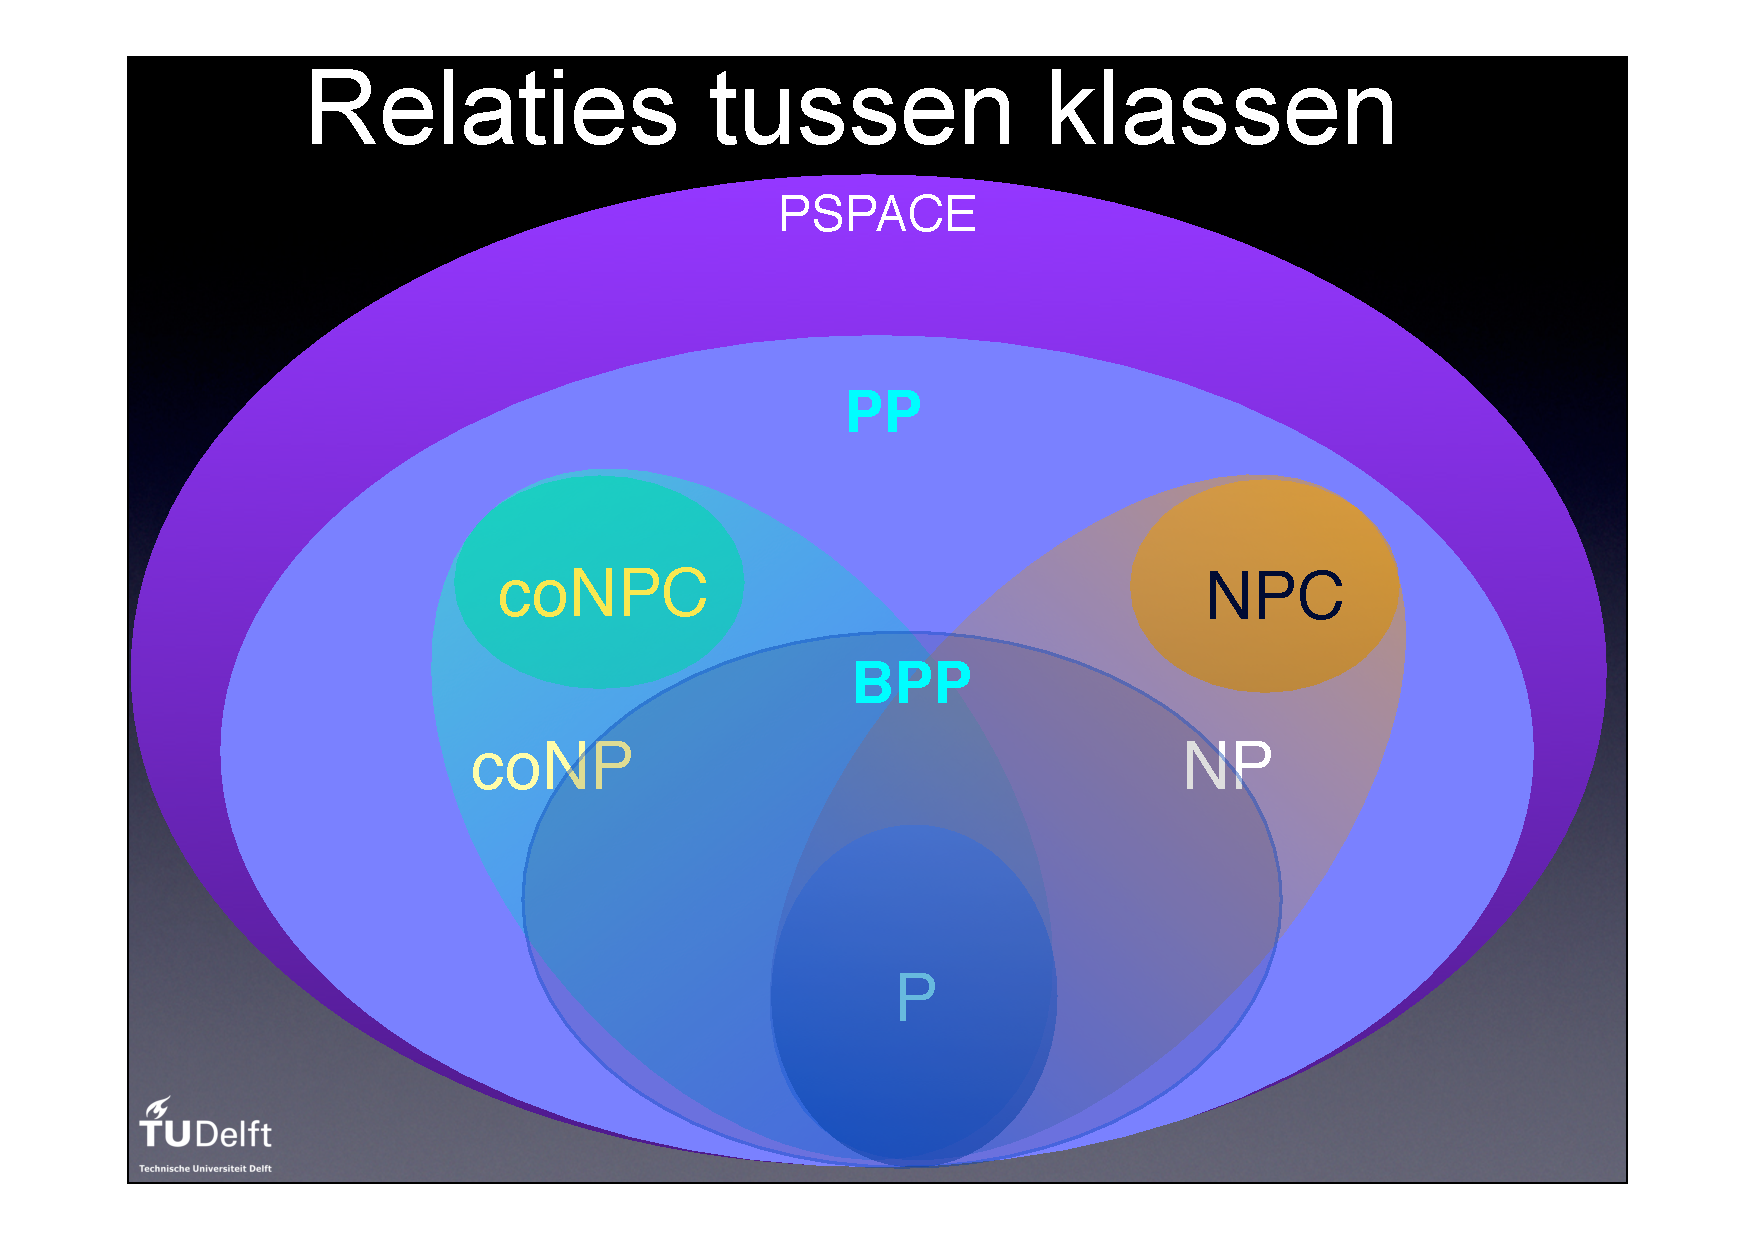
\includegraphics[width=0.6\columnwidth]{slides/bpp}
\end{figure}

\section*{Mind changing machines}

\textbf{n-trial machines} zijn TMs die n verschillende outputs (achter elkaar) mogen geven en waarbij de laatste output als resultaat van de berekening telt.

%Voor elke $n$ is er een functie $f$ zodat $f$ niet geidentificeerd kan worden door een n-trial machine, maar wel door een n+1-trial machine.

\section*{P $\not=$ NP}

\begin{description}
\item[Church-Turing These (CTT):] ieder fysisch realiseerbaar berekeningsproces kan worden gesimuleerd met een deterministische Tm.
\item[Sterke Church-Turing These (SCTT):] ieder fysisch realiseerbaar efficient berekeningsproces kan worden gesimuleerd met een deterministische Tm en met polynomiale overhead.
\item[Sterke P $\not=$ NP These (SPNPT):] een NP-hard probleem kan niet worden opgelost door een fysisch proces in polynomiale tijd.
\end{description}

\section*{Quantum Computers}

\begin{itemize}
\item Quantum computers opereren op quantum bits (qubits). Een qubit kent twee basistoestanden:
\begin{itemize}
\item spin-down ( $|0\rangle$)
\item spin-up ( $|1\rangle$ )
\end{itemize}
\item Superstate $|\psi\rangle$ is een lineaire combinatie van de basistoestanden:
\begin{itemize}
\item $|\psi\rangle = a |0\rangle + b|1\rangle$ met waarschijnlijkheidsamplituden a, b $\in \mathbb{C}$
\item Meting van een qubit state $|\psi\rangle$ resulteert altijd in een basistoestand $|0\rangle$ of $|1\rangle$.
\item Deze toestanden treden op met waarschijnlijkheid $|a|^2$ , respectievelijk $|b|^2$ \\
(hieruit volgt dat $|a|^2$ + $|b|^2$ = 1)
\end{itemize}
\item Een quantum systeem van $n$ qubits kent $2^n$ basistoestanden. Een superpositie toestand $|\psi\rangle$ is te schrijven als $|\psi\rangle$ = $a_1|000...0\rangle + a_2|000...1\rangle + ... + a_{2^n}|111...1\rangle$ met $\Sigma_{i=1..2^n} |a_i|^2 = 1$.
\item Een quantumberekening is een serie lineaire transformaties van superposities.
\end{itemize}

\textbf{BQP} is de klasse van alle problemen waarvoor een quantum computer het juiste antwoord geeft in polynomiale tijd met kans $\geq$ 0.667

\textbf{Relaties:} P $\subseteq$ BPP $\subseteq$ BQP $\subseteq$ PP $\subseteq$ PSPACE

\begin{figure}[H]
\centering
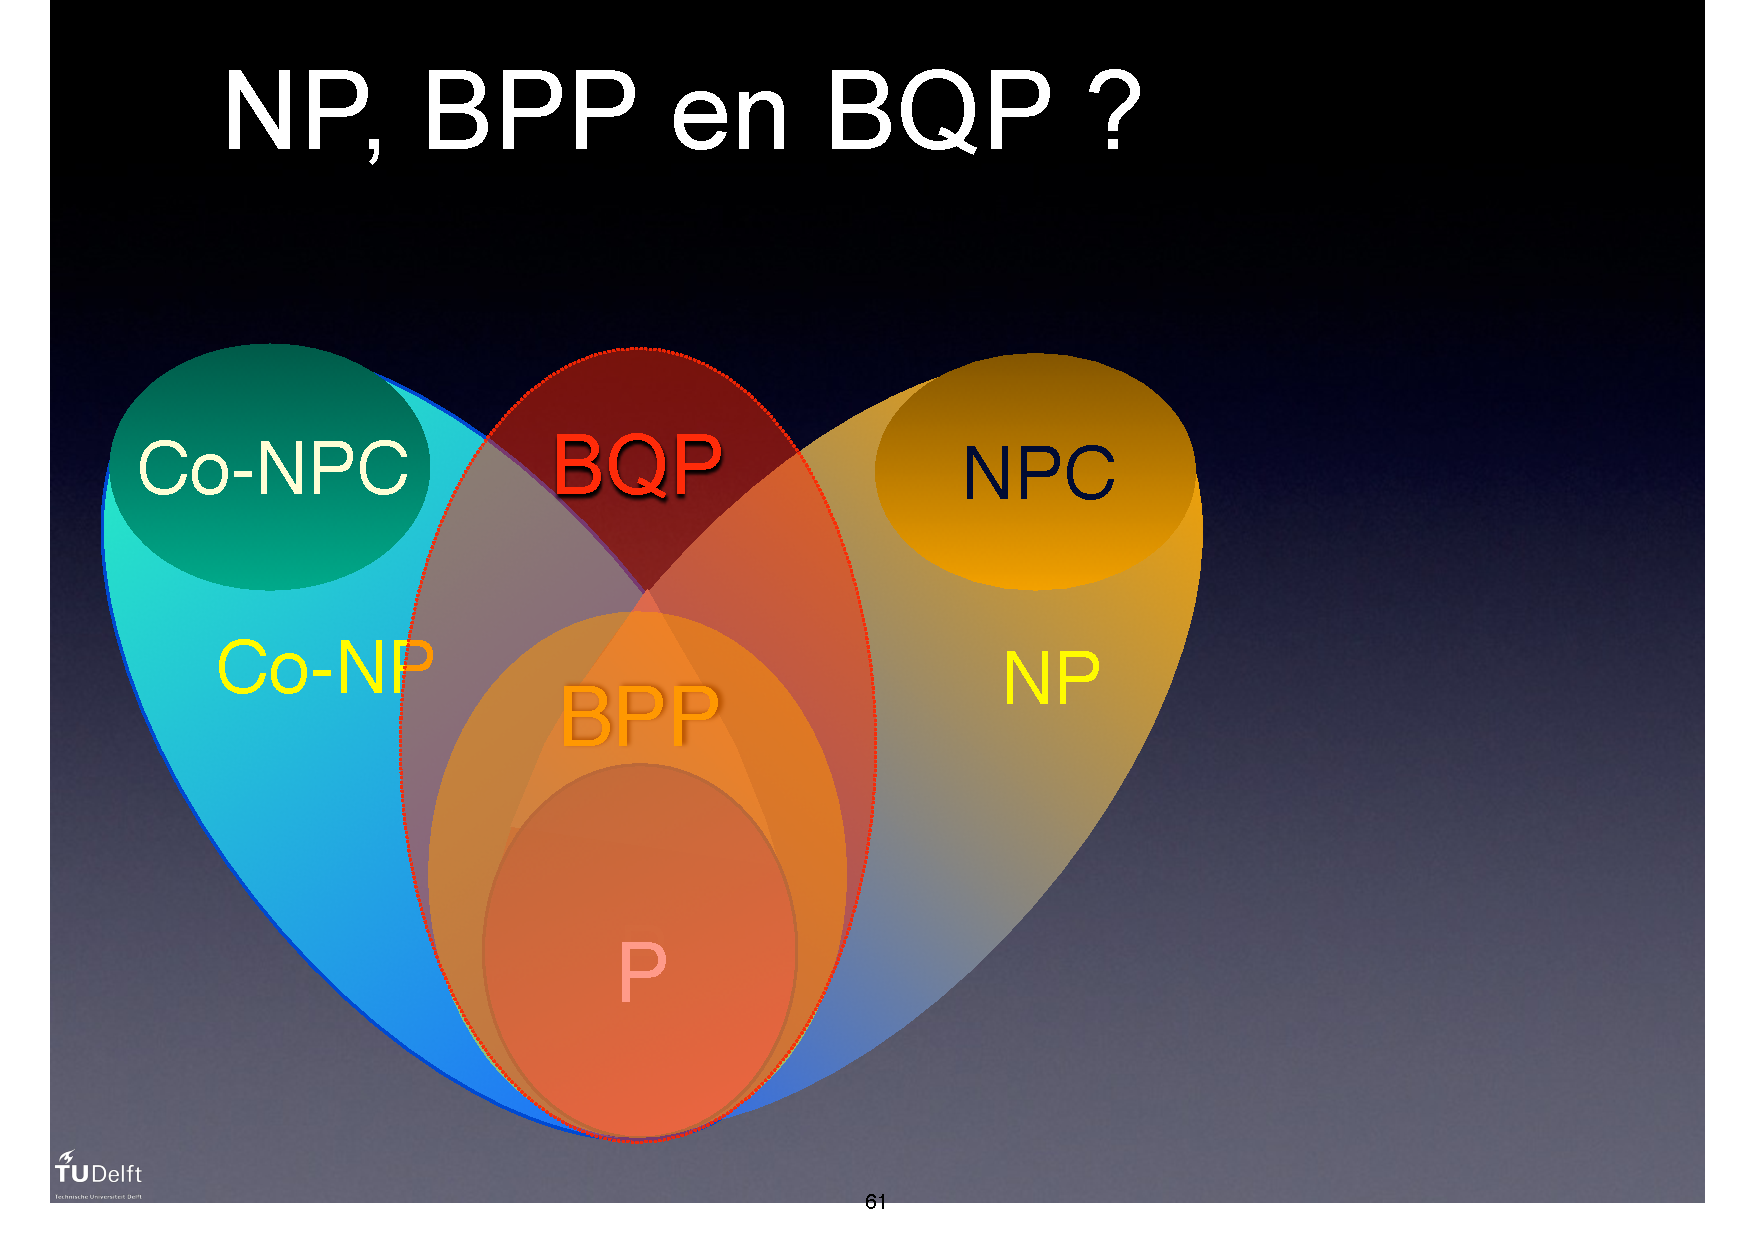
\includegraphics[width=0.6\columnwidth]{slides/bqp}
\end{figure}

\begin{itemize}
\item Soms wordt met quantum computing exponenti\"ele versnelling bereikt. (Shor's Algoritme)
\item Voor aantal problemen kan met quantum computing ``slechts'' een kwadratische versnelling worden bereikt. (Grover's Algoritme)
\item Er zijn voldoende redenen om de Sterke Church Turing These als verworpen te beschouwen op grond van resultaten behaald met quantum computing.
\item Er zijn geen redenen om de Sterke P $\not=$ NP These te verwerpen: ook quantum computing is er (nog) niet in geslaagd NPC problemen in polynomiale tijd op te lossen.
\end{itemize}

\end{document}
